\documentclass{article}

\usepackage[a4paper, left=1.5cm, right=1.5cm, top=2cm, bottom=2cm]{geometry}

\usepackage{../../../../components/components}

\usepackage{hyperref}
\usepackage{fancyhdr}


% Configuration des en-têtes et pieds de page
\pagestyle{fancy}
\fancyhf{} % reset tout

\fancyhead[L]{DL3 Math-Info GA5}
\fancyhead[C]{Théorie des groupes}
\fancyhead[R]{2026-2027}

\fancyfoot[L]{Ewen Rodrigues de Oliveira}
\fancyfoot[R]{\thepage}

\begin{document}

\docTitle{Chapitre 2 : Groupes quotients}

\section{Relations d'équivalence et classes d'équivalence}

\definition{Soit \(E\) un ensemble. Soit \(R\) (un sous-ensemble de \(E \times E\)) une relation.\\
On pose \(xRy \Leftrightarrow (x, y) \in R\) et on dit que \(x\) est en relation avec \(y\) par \(R\).}
\theorem{Propriété}{Relation d'équivalence}{true}{
    Soit \(R\) une relation sur \(E\). On dit que \(R\) est une \textbf{relation d'équivalence} si :
    \begin{itemize}
        \item \(R\) est réflexive : \( \forall x \in E, xRx\).
        \item \(R\) est symétrique : \( \forall x, y \in E, xRy \Rightarrow yRx\).
        \item \(R\) est transitive : \( \forall x, y, z \in E, (xRy \wedge  yRz) \Rightarrow xRz\).
    \end{itemize}
}


\definition{Soit \(R\) une relation d'équivalence sur \(E\). Pour \(x \in E\), on appelle \textbf{classe d'équivalence} de \(x\) et on note \(\overline{x}\) (ou \([x]_R\) ou \(x+k\mathbb{Z}\)) l'ensemble \(\{ y \in E \mid xRy \}\).}


\theorem{Proposition}{}{true}{Si deux classes d'équivalence ont un élément en commun, alors elles sont égales.}

\definition{Soit \((F_i)_{i \in I}\) une famille de parties de \(E\). On dit que cette famille est une \textbf{partition} de \(E\) si :
\begin{itemize}
    \item \(E = \bigcup_{i \in I} F_i\) (la réunion des \(F_i\) est \(E\)).
    \item \( \forall i, j \in I, i \neq j \Rightarrow F_i \cap F_j = \emptyset\) (les \(F_i\) sont deux à deux disjointes).
\end{itemize}}

\illustration{On peut reprendre l'idée intuitive d'un univers en probabilités :

    \begin{center}
        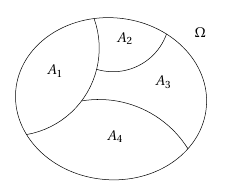
\includegraphics[width=0.25\textwidth]{./images/partition.png}
        \captionof{figure}{Partition de \(\Omega\) en \(A_1, A_2, A_3, A_4\)}
    \end{center}
}
\theorem{Proposition}{}{false}{Les classes d'équivalence d'une relation d'équivalence \(R\) forment une partition de \(E\).}
\noindent{
    \textbf{Preuve:}
    \begin{itemize}
        \item Les classes sont non vides.
        \item Deux classes différentes sont disjointes (elles n'ont pas d'élément en commun).
        \item L'union des classes est \(E\). $\Box$ 
    \end{itemize}
}

\theorem{Proposition}{}{false}{
    Soit \((F_i)_{i \in I}\) une partition de \(E\). On peut définir une relation d'équivalence \(R\) sur \(E\) par : \(xRy \Leftrightarrow \exists i \in I : x,y\in F_i\).\\
    Alors \(R\) est d'équivalence.
}

\noindent\textbf{Preuve:}\\
\begin{itemize}
    \item \textit{Réflexivité :} Soit \(x \in E\). Par définition de partition, \(\exists i \in I\) tel que \(x \in F_i\). Donc \(xRx\).
    \item \textit{Symétrie :} Soient \(x, y \in E\) tels que \(xRy\). Par définition de \(R\), \(\exists i \in I\) tel que \(x, y \in F_i\). Donc \(y, x \in F_i\) et ainsi \(yRx\).
    \item \textit{Transitivité :} Soient \(x, y, z \in E\) tels que \(xRy\) et \(yRz\). Par définition de \(R\), \(\exists i, j \in I\) tels que \(x, y \in F_i\) et \(y, z \in F_j\). Comme \(y \in F_i\) et \(y \in F_j\), on a \(F_i \cap F_j \neq \emptyset\). Par définition de partition, on en déduit que \(i = j\). Donc \(x, z \in F_i\) et ainsi \(xRz\). $\Box$
\end{itemize}

\definition{
    Soit \(R\) une relation d'équivalence sur \(E\).\\
    On appelle \textbf{ensemble quotient} de \(E\) par \(R\) et on note \(E/R\) l'ensemble des classes d'équivalence de \(R\).\\
    \textit{i.e.  \(E/R = \{ \overline{x} \mid x \in E \}\).}
}

\definition{
    Soit \(f : E \to F\) une application. \\
    On dit que f \textbf{passe au quotient} si \( \forall x, y \in E \text{ avec } xRy \Rightarrow f(x) = f(y)\).
}

\definition{
    Soit \(S \subseteq E\). On dit que \(S\) est un \textbf{système de représentants} pour \(R\) si pour toute classe \(C\) de \(R\), il existe un unique élément dans \(S \cap C\).
}

\section{Congruences}

\subsection{Rappels et généralités}

\definition{Soit \(k \in \mathbb{Z}\). 
On pose la relation \(\equiv_k\) sur \(\mathbb{Z}\) définie par : \(x \equiv_k y \Leftrightarrow y - x \in k\mathbb{Z}\) (i.e. \(k\) divise \(y - x\)).\\
On écrit aussi \(x \equiv y [k]\). \textit{i.e. \(\exists n \in \mathbb{Z}, y - x = kn\)}.
}

\vocabulary{
    \(\equiv_k\) est appelée \textbf{congruence modulo \(k\)}.
}

\theorem{Proposition}{Equivalence}{false}{
    \(\equiv_k\) est une relation d'équivalence sur \(\mathbb{Z}\).
}

\noindent\textbf{Preuve:}\\
\carreaux{10}


\theorem{Proposition}{\(\mathbb{Z}/k\mathbb{Z}\)}{false}{
    On a que \(\mathbb{Z}/\equiv_k = \{ \overline{0}, \overline{1}, \overline{2}, ..., \overline{k-1} \}\) noté \(\mathbb{Z}/k\mathbb{Z}\).\\

    En particulier, \{0, 1, 2, ..., k-1\} est un système de représentants pour \(\equiv_k\).
}
\noindent{
    \textbf{Preuve:}\\
    Soit \(x \in \mathbb{Z}\).\\
    Par la division euclidienne, \(\exists ! (q, r) \in \mathbb{Z} \times \{0, 1, 2, ..., k-1\}\) tel que \(x = kq + r\). Donc \(x - r = kq \in k\mathbb{Z}\) et ainsi \(x \equiv_k r\).\\
    Il reste à voir que \(\overline{i} \neq \overline{j}\) si \(i\neq j\) avec \(i, j \in \{0, 1, 2, ..., k-1\}\).\\
    En effet, \(i-j \in \{ 1-k, 2-k, ..., -1, 1, 2, ..., k-1 \}\) et \(i-j \neq 0\). \\
    Donc \(i-j \notin k\mathbb{Z}\) et ainsi \(i \not\equiv_k j\) donc \(\overline{i} \neq \overline{j}\). $\Box$
}

\theorem{Lemme}{}{false}{
    Soient \(x,y\in \mathbb{Z}\).\\
    Considérons \(\overline{x+y} \in \mathbb{Z}/k\mathbb{Z}\). Alors \(\overline{x+y}\) ne dépend que de \(\overline{x}\) et \(\overline{y}\).\\
    Autrement dit : \(\mathbb{Z} \to \mathbb{Z}/k\mathbb{Z}, x \mapsto \overline{x+y} \text{ et } y \mapsto \overline{x+y}\) passent au quotient.
}
\noindent\textbf{Preuve:}\\
\carreaux{10}


\theorem{Théorème}{\(\mathbb{Z}/k\mathbb{Z}\)}{false}{
On a que \((\mathbb{Z}/k\mathbb{Z}, +)\) est un groupe abélien. 
}
\newpage
\noindent\textbf{Preuve:}\\
\carreaux{7}

\theorem{Proposition}{\(\mathbb{Z}/k\mathbb{Z}\)}{false}{
Le groupe \((\mathbb{Z}/k\mathbb{Z}, +)\) est le groupe des entiers modulo \(k\).
}
\theorem{Proposition}{\(\mathbb{Z}/k\mathbb{Z}\)}{false}{
Le groupe \((\mathbb{Z}/k\mathbb{Z}, +)\) est cyclique et engendré par \(\overline{1}\).
}

\noindent{\textbf{Preuve:}\\
Le sous-groupe engendré par \(\overline{1}\) est \(\{ \overline{n} \mid n \in \mathbb{Z} \} = \{\overline{n\cdot 1} \mid n \in \mathbb{Z} \} = \mathbb{Z}/k\mathbb{Z}\). $\Box$
}



\newpage
\tableofcontents 
\end{document}

